\subsection{Handcrafting and Customization}
\begin{frame}{What do these examples have in common?}
	\begin{mycolumns}[columns=3,widths={35,28},animation=none]
		\pic[width=\linewidth,trim=25 200 25 25,clip]{wedding}
		
		\pic[width=\linewidth]{shoes}
	\mynextcolumn
		\pic[width=\linewidth,trim=85 0 0 0]{eiffel-tower}
	\mynextcolumn
		\pic[width=\linewidth,trim=70 35 0 0]{draisine}
		
		~
		
		\uncover<2->{\mydefinition{Customization \deutschertitel{Maßschneiderung}}{
			\begin{itemize}
			\item aka.\ handcrafting
			\item labor-intensive production
			\item highly individual goods
			\end{itemize}
		}}
	\end{mycolumns}
\end{frame}

\begin{frame}{Customization of Elevators}
	\begin{mycolumns}[columns=4,T]
		\centering\pic[width=\linewidth]{elevator1-out}

		two buttons
	\mynextcolumn
		\centering\pic[width=\linewidth]{elevator2-out2}

		one button
	\mynextcolumn
		\centering\pic[width=\linewidth]{elevator3-out}

		keyhole
	\mynextcolumn
		\centering\pic[width=\linewidth]{elevator2-out1}

		floor display
	\end{mycolumns}
\end{frame}

\begin{frame}{Customization of Elevators}
	\begin{mycolumns}[columns=4,widths={28,21,28,21},T]
		\centering\pic[width=\linewidth]{elevator1-in2}

		no button to close door
	\mynextcolumn
		\centering\pic[width=\linewidth]{elevator3-in1}

		two keyholes
	\mynextcolumn
		\centering\pic[width=\linewidth]{elevator4-in}

		keycard
	\mynextcolumn
		\centering\pic[width=\linewidth]{elevator2-in2}

		double tap for~undo
	\end{mycolumns}
\end{frame}

\subsection{Mass Production}
\begin{frame}{\myframetitle}
	\begin{mycolumns}
		\mydefinition{Mass Production \deutschertitel{Massenproduktion}\mysource{\fospl\mypages{3--4}}}{
			\begin{itemize}
			\item consequence of industrialization
			\item goods are produced from standardized parts
			\item improved productivity wrt.\ handcrafting
			\item reduced costs, improved quality
			\item but: (almost) no individualism
			\end{itemize}
		}
		\myexample{Principle: One Size Fits All}{
			\begin{itemize}
			\item t-shirts: XS, S, M, L, XL, XXL
			\item swiss-army knife \deutsch{Eierlegende Wollmilchsau}
			\end{itemize}
		}
		\centering\pic[width=.5\linewidth]{wollmilchsau}
	\mynextcolumn
		\vspace{-8mm}
		\pic[width=\linewidth]{swiss-army-knife}
		\mynote{Mass Production for Software?\mysource{\fospl\mypage{7}}}{\mycite{The idea is to provide software that satisfies the
		needs of most customers, which leads almost automatically to the situation, in which customers miss desired functionality and are overwhelmed with functionality they do not need actually (just think of any contemporary office or graphics program). It is often this generality that makes software complex, slow, and buggy.}}
	\end{mycolumns}
\end{frame}
% industrial revolution/era:
% - John Hall, exchangable parts 1826, 25 years of trials (source?)
% - Henry Ford/Ransom Olds, production/assembly line, 1901 (source?)
% - 1961 first industrial roboter at General Motors
% - 1980s automatic assembly lines

\subsection{Mass Customization}
\begin{frame}{About Every Second Car is Unique}
	\centering\pic[width=.66\linewidth]{many-cars}
\end{frame}
\begin{frame}{\myframetitle\ \deutschertitel{Kundenindividuelle Massenproduktion}}
	\begin{mycolumns}[widths={45}]
		\mydefinition{Mass Customization\mysource{\fospl\mypage{4}}}{
			\begin{itemize}
			\item = mass production + customization
			\item customized, individual goods at costs similar to mass production
			\end{itemize}
		}
	
		\myexampletight{Car Configuration}{\pic[width=\linewidth]{toyota-aygo-wheels}}
	\mynextcolumn
		\myexampletight{Car Production}{\pic[width=\linewidth,trim=0 50 0 240,clip]{car-manufacturing}}
		
		\myexample{Other Domains}{bikes, computers, electronics, tools, medicine, clothing, food, financial services, \ldots, software?}
	\end{mycolumns}
\end{frame}

\begin{frame}{Mass Customization for Software?}
	\begin{mycolumns}
		\mydefinition{Mass Customization for Software?}{
			\begin{itemize}
			\item customization: individual software developed using Waterfall model or Scrum
			\item mass production: standard software developed once for millions or billions of users (e.g., Whatsapp messenger)
			\item mass customization: software product lines
			\end{itemize}
		}
	
		\mynote{Why Software Product Lines?}{
			\begin{itemize}
			\item resource limitations: memory, performance, energy
			\item different hardware
			\item different laws
			\item goal: avoid expensive customization
			\end{itemize}
		}
	\mynextcolumn
		\pic[width=\linewidth,page=24]{lego}
	\end{mycolumns}
\end{frame}

\subsection{Recap: The Software Life Cycle}
\begin{frame}{The Project Cartoon}
	\renewcommand{\projectcartoonwidth}{.135}
	\uncover<2-|handout:1-2>{\alt<-8|handout:1>{\hprojectcartoon{01}{how the customer explained it}}{\alt<9|handout:2>{\hprojectcartoon{01}{Requirements}}{\projectcartoon{01}{Requirements}}}}% requirements
	\uncover<3->{\alt<-8,10-|handout:1>{\hprojectcartoon{02}{how the project leader understood it}}{\projectcartoon{02}{how the project leader understood it}}}% modeling
	\uncover<4->{\alt<-8,10-|handout:1>{\hprojectcartoon{03}{how the analyst designed it}}{\projectcartoon{03}{how the analyst designed it}}}% architecture and design
	\uncover<5->{\alt<-8,10-|handout:1>{\hprojectcartoon{04}{how the programmer implemented it}}{\projectcartoon{04}{how the programmer implemented it}}}% implementation
	\uncover<6->{\alt<-8,10-|handout:1>{\hprojectcartoon{05}{what the beta testers received}}{\projectcartoon{05}{what the beta testers received}}}% testing
	\uncover<7->{\alt<-8,10-|handout:1>{\hprojectcartoon{10}{how it was supported}}{\projectcartoon{10}{how it was supported}}}% maintenance
	\uncover<8->{\alt<-8|handout:1>{\hprojectcartoon{13}{what the customer really needed}}{\alt<9>{\hprojectcartoon{13}{Product}}{\projectcartoon{13}{Product}}}}% customer / SE II
	\\
\end{frame}

\begin{frame}{\myframetitle}
	\waterfallcartoon\\
\end{frame}

\subsection{Features and Products of a Domain}
\begin{frame}{What is a Feature?}
	\begin{mycolumns}[widths={45},t]
		\uncover<2->{\mydefinition{Feature \deutsch{Feature} \mysource{\fospl\mypage{18}}}{\mycite{A \emph{feature} is a characteristic or end-user-visible behavior of a software system.}}}
		\centering\xkcd{2369}{width=.9\linewidth,trim=35 35 35 35,clip}
	\mynextcolumn
		\uncover<3->{\mynote{Feature in a Product Line \mysource{\fospl\mypage{18}}}{\mycitebegin Features are used in product-line engineering
			\begin{itemize}
				\item to specify and communicate commonalities and differences of the products between stakeholders \deutsch{Akteure} and
				\item to guide structure, reuse, and variation across all phases of the software life cycle.\myciteend
			\end{itemize}
		}}
		\renewcommand{\projectcartoonwidth}{.18}\scriptsize
		\uncover<4->{\waterfallcartoon}\\
	\end{mycolumns}
\end{frame}
% TODO picture of a program highlighting one or two features? settings? changelog? marketing description of new features (Github?)?

% goals of features
%a distinctively identifiable functional abstraction that must be implemented, tested, delivered, and maintained” (Kang et al.
%a product characteristic from user or customer views, which essentially consists of a cohesive set of individual requirements” (Chen et al.
%an optional or incremental unit of Zave 2003) 

\begin{frame}{What is a Product?}
	\begin{mycolumns}[t]
		\mydefinition{Product \deutsch{Produkt} \mysource{\fospl\mypage{19}}}{\mycite{A \emph{product of a product line} is specified by a valid feature selection (a subset of the features of the product line). A feature selection is \emph{valid} if and only if it fulfills all feature dependencies.}}
		
		\mynote{Note on Terminology}{
			\begin{itemize}
				\item in this course:
				
					product = product variant = variant
				\item software product: a product consisting only of software
				\item software is more than a program: requirements, models, source code, tests, documentation
				\item this course focuses on source code
			\end{itemize}
		}
		% TODO exemplify difference between hardware product, software product (VLC?), and program (reuse pictures from before)
	\mynextcolumn
		\myexampletight{Product Map for Eclipse (excerpt)}{
			\pic[width=\linewidth,trim=0 460 635 0,clip]{eclipse-product-map}
		}
	\end{mycolumns}
\end{frame}
% TODO Venn diagram could also be a good visualization: products correspond to sets and features to set elements

\begin{frame}{What is a Domain?}
	\begin{mycolumns}
		\mydefinition{Domain \deutsch{Domäne} \mysource{\fospl\mypage{19}}}{ % TODO cite CE00 here too?
			\mycitebegin A \emph{domain} is an area of knowledge that:
			\begin{itemize}
				\item is scoped to maximize the satisfaction of the requirements of its stakeholders,
				\item includes a set of concepts and terminology understood by practitioners in that area,
				\item and includes the knowledge of how to build software systems (or parts of
				software systems) in that area.\myciteend
			\end{itemize}
		}
		\mynote{Features of a Domain}{
			\begin{itemize}
				\item a feature is a domain abstraction
				\item identification of features in a domain requires domain expertise
				\item later: select features for a product line?
			\end{itemize}
		}
	\mynextcolumn
		\pic[width=.5\linewidth]{many-cars}

		\hfill\xkcd{2369}{width=.5\linewidth,trim=35 35 35 35,clip}\hfill{}

		\hfill\pic[width=.5\linewidth]{eclipse-luna}
	\end{mycolumns}
\end{frame}
% TODO add more examples for domains

\subsection{Software Product Line}
\begin{frame}{\myframetitle}
	\begin{mycolumns}[widths={78},columns=1]
		\mydefinition{Software Product Line \mysource{\seiwhitepaperspl\mypage{5}}}{\mycitebegin A \emph{software product line} is 
			\begin{itemize}
				\item a set of software-intensive systems \uncover<2->{\myexampletight{}{aka.\ products or variants}}
				\item that share a common, managed set of features \uncover<3->{\myexampletight{}{common set, but not all products have all features in common}}
				\item satisfying the specific needs of a particular market segment or mission \uncover<4->{\myexampletight{}{aka.\ domain \deutsch{Domäne}}}
				\item and that are developed from a common set of core assets in a prescribed way.\myciteend \uncover<5->{\myexampletight{}{aka.\ planned, structured reuse \deutsch{Wiederverwendung}}}
				\mysource{\href{https://resources.sei.cmu.edu/library/asset-view.cfm?assetID=513819}{Software Engineering Institute, Carnegie Mellon University}}
			\end{itemize}
		}
	\end{mycolumns}
\end{frame}
% variants / platforms / domain / variant generation
% configurable software, highly-configurable software, variable software, software variation

\subsection{Product-Line Engineering}
\begin{frame}{\myframetitle}
	\begin{mycolumns}
		\mydefinition{Product-Line Engineering\mysource{\sple\mypage{14}}}{
			\mycite{\emph{Software product-line engineering} is a paradigm to develop software applications (software-intensive systems and software products) using software platforms and mass customization.}
%			\begin{itemize}
%			\item aka.\ product-line development \mysource{\seiwhitepaperspl\mypage{207}}
%			\end{itemize}
		}
		\mynote{Promises of Product Lines \mysource{\fospl\mypages{9--10}}}{
			\begin{itemize}
				\item tailor-made \deutsch{Maßschneiderung}
				\item reduced costs \deutsch{Kostenreduzierung}
				\item improved quality \deutsch{Qualitätssteigerung}
				\item reduced time-to-market \deutsch{Reduzierung der Produktentwicklungszeit}
			\end{itemize}
		}
	\mynextcolumn
		\vspace{-5mm}
		\mynotetight{Idea of Product-Line Engineering}{
			Reduce effort per product by means of an up-front investment for the product line:
			
			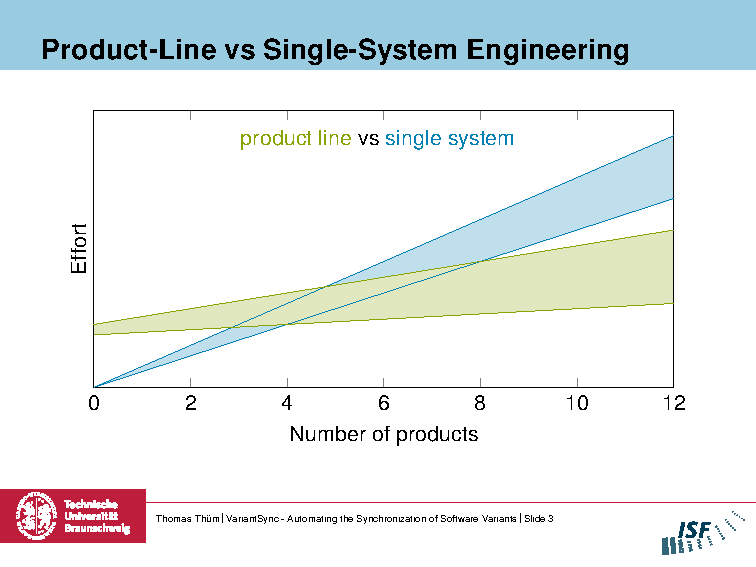
\includegraphics[width=\linewidth,trim=30 60 30 50,clip]{product-line-vs-single-system}
		}
		\mydefinition{Single-System Engineering}{
			\begin{itemize}
			%\item aka.\ single-system development \mysource{\seiwhitepaperspl\mypage{7}}
			\item \deutsch{Einzelsystementwicklung}
			\item classical software development that is not considered as product-line engineering
			\end{itemize}
		}
	\end{mycolumns}
\end{frame}

% product-line hall of fame
% success stories: Boing, Bosch, Hewlett Packard, Toshiba, General Motors \mysource{\fospl}

% TODO \subsection{Running Examples?}
% \fospl: data management for embedded systems, product line of a graph library

% not software, not running: financial services (or in \lecturemodeling?), bikes, shoes, notebooks, ...
% Linux, Graph Product Line \lectureruntime\ or \lecturecloneandown, Configurable Database, Elevator Product Line, Printer product lines, Car configurators, software ecosystem (Browser plug-ins, IDE plug-ins)

% elevators: pictures from various elevators (OVGU, UULM, Bern), invisible end-user-visible features (e.g., double click for deselection)
% if you do this at home: do not select all stops before you know it is working

% how many examples in first lecture? move certain examples in later lectures? if so, which ones?
%\subsection{Automotive Systems}
% car configurators
% history? number of variants over time?
%\subsection{Notebooks}
% lenovo, microsoft, apple
%\subsection{Printer (Firmware)}
% real printers, 3d printers
% 30 printers per year, more examples
% XKCD: all-in-one paper processor
%\subsection{Operating Systems}
% windows, linux!!!, android
% Linux: where is it used? on which principal hardware? how many instances are running world wide? how many commits and developers? how many versions have been release and since when? screenshot how it looks like when linux is configured
% apps?
%\subsection{Integrated Development Environments}
% eclipse
%\subsection{Browsers}
% plug-ins

% apps! in market store android, iOS
% ecos, packages in debian

%\subsection{Beyond Software}
% financial products by KfW, bikes, shoes, muesli, Subway, headphones, lego, detergents, furniture (handcrafted vs standardized vs product line), kitchens
% brompton: picture in ulm slides

% zoo of animals/tools

% historical development? exchangable parts, production lines, automated product lines, ...
% all-in-one solution vs custom development? software for German fire departments
% all-in-one application software vs embedded software
% reasons for custom development: 

% goal of the lecture

%\subsection{Features}

%\subsection{Software Product Lines}
%% product-line engineering
%\begin{frame}{Who Produces Only One Product?}
%	\href{https://pxhere.com/en/photo/920906}{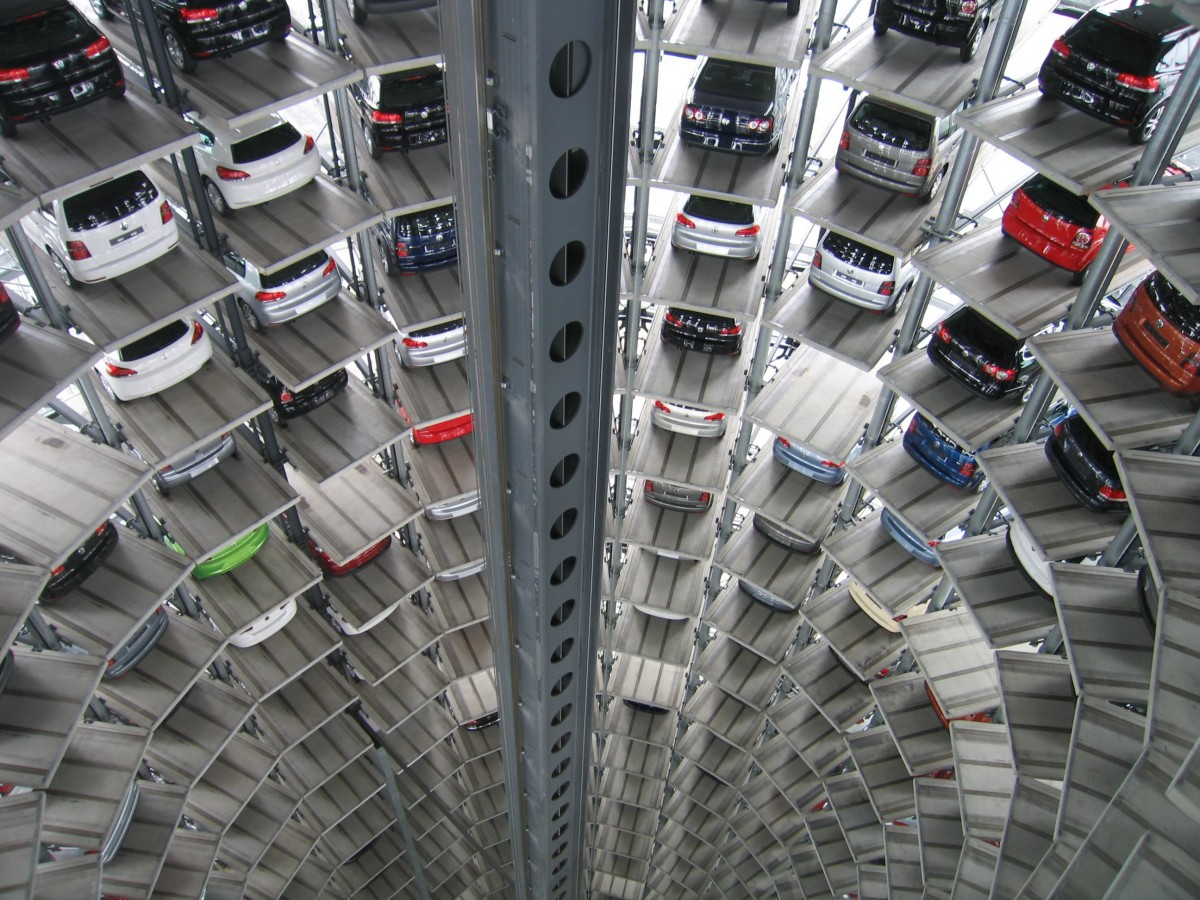
\includegraphics[width=.6\linewidth]{car-tower}}
%\end{frame}

%\subsection{Single System}
%% single-system engineering
%
%\begin{frame}{Greenfield Development? \deutschertitel{Auf der grünen Wiese?}}
%	\href{https://github.com/SoftVarE-Group/SlideTemplate/blob/main/pics/nature/may21-ulm.jpg}{\includegraphics[width=.6\linewidth]{may21-ulm}}
%\end{frame}



% add illustration for variants/versions (space/time) by icons of word/excel/powerpoint/one note/... over the years




% Apel 2013, Page 49
%Compile-time variability is decided before or at compile time.
%Load-time variability is decided after compilation when the program is started.
%With run-time variability, decisions can be made and changed during program
%execution.



% explain configurators vs selectors? for example, iPhone is available is produced in any combination and then selled, still there are selectors to find the right product easily. cf. ebay/amazon




% history on product lines? how old are product lines and ideas discussed in this lecture?




